\subsection{Stereografische Projektion}
\label{sec:stereo}
Die stereografische Projektion ist eine winkeltreue Projektion. Sie ist allerdings nicht flächentreu.
Man kann mit dieser Projektion die ganze Erde abbilden allerdings nimmt die Verzerrung sehr schnell stark zu, weshalb die stereografische Projektion  für globale Abbildungen eher ungeeignet ist. Diese Projektion erhält man, wenn man von einem Ausgangspunkt geraden durch jeden Punkt der Erde zieht, die Schnittpunkte dieser Geraden mit der Projektionsebene sind die Punkte auf die projiziert wird.
Die Projektionsebene kann grundsätzlich frei positioniert werden.\\

\begin{figure}[hbtp]
\centering
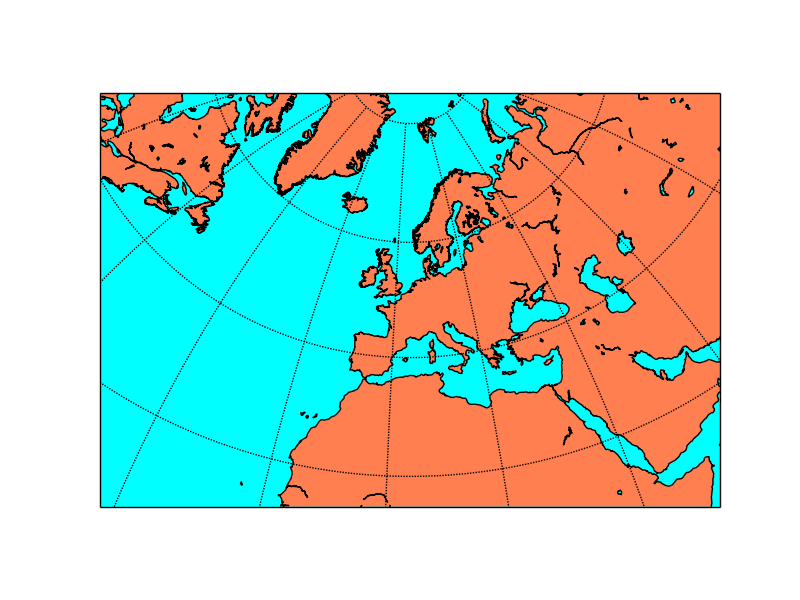
\includegraphics[scale=0.5,origin=c]{/Users/student/seminar/Kartendarstellungen/seminar/stere} \caption{Stereografische Projektion}
\end{figure}
\newpage 